\chapter{图神经网络辅助深度强化学习的非理想硬件去蜂窝大规模 MIMO 系统}\label{chap:MIMOLP}
在去蜂窝大规模多输入多输出（CF‑mMIMO）系统中，通过密集部署大量接入点（AP）可实现无缝通信覆盖，显著提升用户的频谱效率（SE）与系统总容量。然而，该方案的实施需要高昂的部署成本，且不可避免地需要采用非理想硬件。本章研究了在用户设备（UE）端使用非线性功率放大器（PA）、接入点端使用低精度模数转换器（ADC）的上行 CF‑mMIMO 系统中，用户可达速率的性能。

具体而言，本章推导了上行用户可达速率的闭合表达式，并综合分析了接入点数量、用户密度、接入点天线数以及 ADC 精度等多种因素的影响。为抑制用户间干扰并最大化和速率，本章提出一种基于图神经网络（GNN）辅助的演员‑评论家算法（DMAGNN‑AC）用于功率分配。所构建的框架克服了深度强化学习在高维非结构化状态空间中的表示瓶颈，并提供具有物理可解释性的特征嵌入。
与全功率发射方案相比，所提功率分配方案可使速率提升近一倍。此外，为缓解低精度 ADC 对速率的不利影响，本章进一步设计了一种增强型算法 —— 多智能体深度 Q 集成网络（MADQIN），以优化 ADC 精度的分配策略。最后，仿真结果验证了所提方案的有效性。
\section{引言}
在 CF‑mMIMO 系统中，随着接入点（AP）的大规模部署，硬件成本与功耗会随天线数量呈线性增长。一方面，采用低成本收发机替代高精度器件是一种可行的解决思路。然而在实际应用中，这类低成本方案会使射频（RF）链路更容易受到各类硬件损伤的影响。另一方面，采用低分辨率模数转换器（ADC）是实现低成本、低功耗 CF‑mMIMO 系统的有效途径，但该方式需要更为精准的信道模型与优化算法来抑制干扰与噪声。
为缓解硬件损伤带来的性能下降，通过优化功率分配以降低用户间干扰是一种有效的策略。传统优化算法如分数规划（FP）和加权最小均方误差（WMMSE）等，在理论层面可实现优异性能，但其过高的计算复杂度难以满足实际部署需求，且难以全面适配实际通信场景中的硬件损伤与信道衰落。相比之下，无模型机器学习方法，尤其是深度强化学习（DRL），凭借其较低的在线计算复杂度与无需先验训练数据集等优势，成为当前研究热点。然而，传统 DRL 难以有效捕捉用户间复杂的干扰关系与空间相关性，通常会导致优化效率偏低。

为突破这一局限，近期相关研究借助图表示方法建模多用户系统中的干扰关系与空间相关性。图神经网络（GNN）能够将原始信道状态信息（CSI）映射为低维图嵌入，显式保留用户间的空间关联特征，从而为 DRL 提供更具表征能力的状态空间。同时，GNN 对动态图结构（如用户移动带来的拓扑时变）的处理能力，与 DRL 的环境交互机制具有天然兼容性，二者深度融合可显著提升系统的移动性管理与网络协同性能。据此，本文提出一种高性价比、工程可实现的 CF‑mMIMO 通信方案，以充分挖掘系统性能潜力；并构建自适应网络优化框架，通过解耦功率分配问题，有效克服传统 DRL 在高维非结构化状态空间中存在的表示瓶颈。
\section{模型设计}
在本文中，我们考虑了一个如图 1 所示的上行链路 CF-mMIMO 系统，该系统由 MN 个天线的接入点（AP）和 K 个单天线的用户设备（UE）组成。所有接入点均通过回程链路与中央处理单元（CPU）相连。该系统采用时分双工（TDD）协议进行数据传输。由于本文仅关注上行数据传输阶段，因此相干时间间隔被分为两个阶段：1）上行链路训练；2）上行数据传输。
\subsection{信道估计}
在本研究中，我们采用了无相关瑞利衰落信道模型[25]。第 m 个接入点与第 k 个用户设备之间的信道增益被表示为

\begin{equation}\mathbf{g} _{mk} = {\beta _{mk}^{1/2} } {{\bf{h}}_{mk}},\end{equation}

它同时考虑了大规模衰落效应$\beta_{mk}$ 和小规模衰落 $\mathbf{h} _{mk}$ 。其中，$\beta_{mk}$ 同时考虑了几何衰减和阴影衰落，并且假定其在相干时间间隔内保持不变。$\mathbf{h} _{mk}$ 的元素是具有瑞利分布包络的复高斯随机变量。设 $\tau_\text{c}$ 为相干间隔的长度，$\tau_\text{p}$ 表示每个相干间隔的上行链路训练时间。由于训练时间长度的限制，我们采用 $\tau_\text{p} < K$ 的非正交导频，并将使用相同导频序列的 UE 集合定义为第 k 个 UE。在上行链路训练阶段，所有 K 个用户同时向所有 AP 发送非正交导频序列。第 k 个 UE 的导频信号可以表示为 $\sqrt{\tau_\text{p}}\boldsymbol{\varphi}_k\in \mathbb{C} ^{\tau_\text{p}\times1}$，其中 $\left\|\boldsymbol{\varphi}_k\right\|^2=1$ 。

本文采用更为精细的硬件非线性确定性行为模型，旨在更准确地建模导致硬件损伤的主要因素\cite{paper1}。该确定性行为模型的主要优势之一在于，其能够通过少量参数表征各类硬件损伤的物理效应。该模型将硬件输入–输出关系描述为\cite{paper2}
\begin{equation}
x_\text{out}=\sum_{i=0}^{N_p}a_{2i+1}x_\text{in}\left | x_\text{in} \right |^{2i}  
\end{equation}
式中，$a_{2i+1}$为模型复系数，非线性阶数可表示为$2N_p + 1$。该模型统一表征了功率放大器、本振、混频器及其他硬件器件的非线性特性。
需要指出的是，对于带内失真，由于偶次项主要出现在带外，准无记忆多项式中仅保留奇次项。此外，三次项能够刻画射频放大器中最主要的非线性来源 \cite {paper3},\cite {paper4}。因此，本文采用 的三次多项式模型。已有研究表明，三次多项式模型具有较高精度，可有效逼近功率放大器的实际非线性特性 \cite {paper5},\cite {paper6}。
经功率放大器非线性作用后，第 k个用户设备的输出信号可表示为
\begin{equation}
\label{eqn-1}\boldsymbol{\phi }_k = \underset{\tilde{a}_1 }{\underbrace{{a_1}\sqrt {{\tau _\text{p}}}} }  \boldsymbol{\varphi }_k + \underset{\tilde{a}_3 }{\underbrace{{a_3}{\tau _\text{p}}\sqrt {{\tau _\text{p}}}} }  \boldsymbol{\varphi} _k{\left\| {\boldsymbol{\varphi }_k} \right\|^2},
\end{equation}
式中，$\tilde{a}_1 \triangleq a_1\sqrt{\tau_\text{p}}$，$\tilde{a}_3 \triangleq a_3\tau_\text{p}\sqrt{\tau_\text{p}}$。第 $m$ 个接入点接收到的导频矩阵为
\begin{equation}\label{eqn-2}
\begin{aligned}
\mathbf{Y}_{\text{p},m} &= \sqrt {{\rho _\text{p}}}\sum_{k=1}^{K}  {{\bf{g}}_{mk}}\boldsymbol{\phi }_k^H + {\mathbf{W}_{\text{p},m}} \\
&= \sqrt {{\rho _\text{p}}}\sum_{k=1}^{K}  ({\tilde{a}_1}{{\bf{g}}_{mk}}\boldsymbol{\varphi} _k^H + \tilde{a}_3 {{\bf{g}}_{mk}}\boldsymbol{\varphi} _k^H{\left\| {\boldsymbol{\varphi }_k} \right\|^2}) + {\mathbf{W}_{\text{p},m}},
\end{aligned}
\end{equation}
式中，$\rho_\text{p}$ 为导频信号的归一化信噪比（SNR）。此外，$\mathbf{W}_{\text{p},m} \in \mathbb{C}^{N \times \tau_\text{p}}$ 表示第 $m$ 个接入点处的加性高斯白噪声（AWGN）矩阵，其第 $\varsigma$ 列满足分布
$\left [ \mathbf{W}_{\text{p},m} \right ] _\varsigma \sim \mathcal{CN} (\mathbf{0},\mathbf{I}_N)$。
本文采用非均匀量化器分析低精度模数转换器（ADC）对系统性能的影响。为此，引入经典的加性量化噪声模型（AQNM），该模型将量化过程引入的失真等效为高斯随机变量。已有研究验证，该模型在中低信噪比条件下具有足够的建模精度\cite{paper7},\cite{paper8}。结合式\eqref{eqn-2}，第 \(m\) 个接入点处ADC的输出可表示为
\begin{align}\label{eqn-3}{\tilde {\bf{Y}}_{\text{p},m}} & \triangleq {\alpha _m}{\mathbf{Y}_{\text{p},m}} + {\tilde {\bf{W}}_{\text{p},m}} \nonumber\\
&= {\alpha _m}\sqrt {{\rho _\text{p}}} \sum_{k=1}^{K}  ({\tilde{a} _1}{{\bf{g}}_{mk}}\boldsymbol{\varphi} _k^H + {\tilde{a}_3}{{\bf{g}}_{mk}}\boldsymbol{\varphi} _k^H{\left\| {\boldsymbol{\varphi}_k} \right\|^2})+ {\alpha _m}{\mathbf{W}_{\text{p},m}} + {\tilde{\bf{W}}_{\text{p},m}},\end{align}
式中，参数 $\alpha_m$ 决定第 $m$ 个接入点处模数转换器（ADC）的量化精度，且由量化比特数 $b_m$ 决定\cite{paper9}。此外，式\eqref{eqn-3}中的 $\tilde{\mathbf{W}}_{\text{p},m}$ 表示第 $m$ 个接入点处的加性高斯量化噪声，该噪声与 $\mathbf{Y}_{\text{p},m}$ 互不相关，其协方差矩阵可表示为
\begin{align}\label{eqn-4}
\mathbf{R}_{\tilde{ \mathbf{W}}_{\text{p},m}} &= \mathbb{E}\left\{ {{\tilde{\mathbf{W}}_{\text{p},m}}\tilde {\mathbf{W}}_{\text{p},m}^H} \right\} \nonumber\\ 
&= {\alpha _m}(1 - {\alpha _m})\text{diag}\left(\mathbb{E}\left\{ {{\mathbf{Y}_{\text{p},m}}\mathbf{Y}_{\text{p},m}^H} \right\} \right). 
\end{align}
在第 \(m\) 个接入点对接收导频信号完成量化后，将量化信号 \(\tilde{\mathbf{Y}}_{\text{p},m}\) 向 \(\boldsymbol{\varphi}_k\) 投影可得
\begin{align}\label{eqn-5}
\check{\mathbf{y} }_{\text{p},mk}&\triangleq {\tilde{\mathbf{Y}}_{\text{p},m}}\boldsymbol{\varphi }_k \nonumber\\
%&= {\alpha _m}\sqrt {{\rho _p}} \mathop \sum \nolimits_{k' = 1}^K ({b_1}{{\bf{g}}_{mk'}}\varphi _{k'}^H + {b_3}{{\bf{g}}_{mk'}}\varphi _{k'}^H{\left| {{\varphi _{k'}}} \right|^2}){\varphi _k} + {\alpha _m}{W_{p,m}}{\varphi _k} + {{\tilde W}_{p,m}}{\varphi _k}\\
&= {\alpha _m}\sqrt {{\rho _\text{p}}}\sum_{k'\in \mathcal{P}_k }^{K}  ({\tilde{a}_1} + {\tilde{a}_3}\tau_\text{p}){{\bf{g}}_{mk}}\nonumber \\
&\quad + {\alpha _m}{\mathbf{W}_{\text{p},m}}\boldsymbol{\varphi}_k + {{\tilde{\mathbf{W}}}_{\text{p},m}}\boldsymbol{\varphi}_k.
\end{align}
基于上述推导，可得如下引理。
引理：
采用最小均方误差（MMSE）方法得到的信道向量 $\mathbf{g}_{mk}$ 估计值可表示为
\begin{equation}\label{eqn-6}
\mathbf{\hat{g} }_{mk} = c_{mk} \mathbf{\check{y} }_{\text{p},mk},
\end{equation}
其中
\begin{align}\label{eqn-7}
{c_{mk}} &= \mathbb{E}\left \{ \mathbf{g}_{mk}^H\mathbf{\check{y} }_{\text{p},mk}   \right \} \left ( \mathbb{E}\left \{  \mathbf{\check{y} }_{\text{p},mk}^H\mathbf{\check{y} }_{\text{p},mk}\right \}   \right )^{-1}   \nonumber \\
%&= \frac{{\sqrt {{\tau _p}{\rho _p}} N{\beta _{mk}}{\alpha _m}({a_1} + {a_3}{\tau _p})}}{{N{\alpha _m}({\tau _p}{\rho _p}({a_1} + {a_3}{\tau _p}){\beta _{mk}} + 1)}}{{\bf{\mathord{\buildrel{\lower3pt\hbox{$\scriptscriptstyle\smile$}} \over y} }}_{p,mk}} \\%
&= \frac{{\sqrt {{\tau _\text{p}}{\rho _\text{p}}} {\beta _{mk}}({a _1} + {a _3}{\tau _\text{p}})}}{{{\tau _\text{p}}{\rho _\text{p}}\sum_{k'\in \mathcal{P}_k }^{K} ({a _1} + {a _3}{\tau _\text{p}})^2{\beta _{mk}} + 1}}.
\end{align}
将信道估计第 \(n\) 个分量的均方值记为
\begin{align}\label{eqn-8}
\gamma_{m k}&=\mathbb{E}\left \{ \left | \left [ \mathbf{\hat{g} }_{mk}  \right ]_n  \right |^2  \right \}\nonumber \\ &=\frac{\tau_\text{p} \rho_\text{p} \alpha_{m} \beta_{m k}^{2}\left(a_{1}+a_{3} \tau_\text{p}\right)^{2}}{\tau_\text{p} \rho_\text{p}\sum_{k'\in \mathcal{P}_k }^{K} \left(a_{1}+a_{3} \tau_\text{p}\right)^2 \beta_{m k}+1}.
\end{align}
令 $\boldsymbol{\tilde{g}}_{mk} = \mathbf{g}_{mk} - \hat{\mathbf{g}}_{mk}$ 为信道估计误差。根据线性最小均方误差（MMSE）估计的性质，$\boldsymbol{\tilde{g}}_{mk}$ 与 $\hat{\mathbf{g}}_{mk}$ 相互独立且服从复高斯分布。因此，信道估计误差向量 $\boldsymbol{\tilde{g}}_{mk}$ 中各元素的均方误差满足
$\left[\boldsymbol{\tilde{g}}_{mk}\right]_n \sim \mathcal{CN}\!\left( 0, \beta_{mk}-\gamma_{mk} \right)$。
\subsection{上行数据传输}
在上行数据传输阶段，所有用户设备（UE）同时向接入点（AP）发送数据 $q_k$，其中满足 $\mathbb{E}\{|q_k|^2\}=1,\forall k$。经用户设备侧功率放大器（PA）的非线性作用后，第 $k$ 个用户设备的输出信号为
\begin{align}
\label{eqn-9}{y_k} &= \sqrt {{\rho _\text{u}}} \left( {{a_1}\sqrt {{\eta _k}} {q_k} + {a_3}\sqrt {{\eta _k}} {q_k}{{\left| {\sqrt {{\eta _k}} {q_k}} \right|}^2}} \right)\nonumber \\ 
&= \sqrt {{\rho _\text{u}}} \left( {{\tilde{a}_{1k}}{q_k} + {\tilde{a}_{3k}}{q_k}{{\left| {{q_k}} \right|}^2}} \right),
\end{align}
式中，$\rho_\text{u}$ 表示各用户设备的最大归一化发射功率，$\tilde{a}_{1k} \triangleq a_1\sqrt{\eta_k}$，$\tilde{a}_{3k} \triangleq a_3\eta_k\sqrt{\eta_k}$。此外，功率控制系数 $\eta_k$（$\forall k$）的选取需满足 $\mathbb{E}\left\{|y_k|^2\right\} \le \rho_\text{u}$。因此，该约束可简化为
\begin{equation}\label{eqn-10}
{\left| {{a_1}} \right|^2}{\eta _k} + 2(a_1^ * {a_3} + {a_1}a_3^ * )\eta _k^2 + 6{\left| {{a_3}} \right|^2}\eta _k^3 \le 1,  \forall k.
\end{equation}
第 \(m\) 个接入点接收到的复基带信号可表示为
\begin{equation}\label{eqn-11}
{{\bf{y}}_{\text{u},m}} = \sqrt {{\rho _\text{u}}} \sum_{k = 1}^K ({\tilde{a}_{1k}}{{\bf{g}}_{mk}}{q_k} + {\tilde{a}_{3k}}{{\bf{g}}_{mk}}{q_k}{\left| {{q_k}} \right|^2}) + {\bf{w}}_{\text{u},m},
\end{equation}
式中，$\mathbf{w}_{\text{u},m}\sim \mathcal{CN}(\mathbf{0},\mathbf{I}_N)$ 表示加性噪声。随后，第 \(m\) 个接入点的接收信号经ADC量化，其量化输出可表示为
\begin{align}\label{eqn-12}{{\bf{\tilde y}}_{\text{u},m}} &= {\alpha _m}{{\bf{y}}_{\text{u},m}} + {{\bf{\tilde w}}_{\text{u},m}} \nonumber\\
&= {\alpha _m}\sqrt {{\rho _\text{u}}} \sum_{k = 1}^K ({\tilde{a}_{1k}}{{\bf{g}}_{mk}}{q_k} + {\tilde{a}_{3k}}{{\bf{g}}_{mk}}{q_k}{\left| {{q_k}} \right|^2}) \nonumber\\
&\quad+ {\alpha _m}{{\bf{w}}_{\text{u},m}} + {{\bf{\tilde w}}_{\text{u},m}},
\end{align}
式中，$\boldsymbol{\tilde w}_{\text{u},m}$ 表示量化噪声，其协方差矩阵可表示为
\begin{align}{\mathbf{R}_{{{{\bf{\tilde w}}}_{\text{u},m}}}} \approx {\alpha _m}(1 - {\alpha _m})\text{diag}(\mathbb{E}\left\{ {{{\bf{y}}_{\text{u},m}}{\bf{y}}_{\text{u},m}^H} \right\}).\end{align}
为检测 $q_k$，各接入点（AP）采用分布式方式，通过低复杂度的匹配滤波合并计算本地数据估计值，随后经前传链路将信号汇总至中央处理单元（CPU）进行聚合与译码。由此，中央处理单元处的接收信号可表示为
\begin{align}\label{eqn-14}
{r_{\text{u},k}} &= \sum_{m = 1}^M {\bf{\hat{g}}}_{mk}^H{{{\bf{\tilde y}}}_{\text{u},m}}\nonumber\\
& = \sqrt {{\rho _\text{u}}}  \sum_{m = 1}^M {\alpha _m}\sum_{k' = 1}^K {\bf{\hat g}}_{mk}^H{\tilde{a}_{1k'}}{{\bf{g}}_{mk'}}q_{k'}  
\nonumber\\& \quad+ \sqrt {{\rho _\text{u}}} \sum_{m = 1}^M {\alpha _m}\sum_{k' = 1}^K {\bf{\hat g}}_{mk}^H{\tilde{a}_{3k'}}{{\bf{g}}_{mk'}}q_{k'} {\left| {q_{k'} } \right|^2}
 \nonumber\\& \quad+ \sum_{m = 1}^M {\bf{\hat g}}_{mk}^H{\alpha _m}{{\bf{w}}_{\text{u},m}} + \sum_{m = 1}^M {{{\bf{\hat g}}}^H_{mk}}{{{\bf{\tilde w}}}_{\text{u},m}}.
\end{align}	
随后，基于 $r_{\text{u},k}$ 对 $q_k$ 进行检测。在下一节中，我们将推导可达速率的闭式表达式。
\subsection{可实现速率分析}
本节在同时考虑功率放大器（PA）非线性与低精度模数转换器（ADC）的条件下，推导了CF-mMIMO系统中上行用户设备的可达速率。由于各接入点仅能获取信道估计信息，中央处理单元（CPU）无法获知真实信道状态。尽管中央处理单元未知当前实际信道状态，但其假设信道状态的均值已知，并利用该已知均值计算可达速率\cite{paper6}。结合式\eqref{eqn-14}，可将中央处理单元的接收信号重新表示为
\begin{align}\label{eqn-15}
{r_{\text{u},k}}& = {\text{ES}_k} \cdot {q_k} + {\text{BU}_k} \cdot {q_k} + \sum_{k' \ne k}^K {\text{I}_{kk'}} \cdot q_{k^\prime} \nonumber \\
&\quad+\sum_{k' \ne k}^K {\text{NB}_{kk'}} \cdot q_{k^\prime}  + {\text{N}_k} + {\text{Q}_k},
\end{align}
式中，$\text{ES}_k$、$\text{BU}_k$、$\text{I}_{kk'}$、$\text{NB}_{kk'}$、$\text{N}_k$ 和 $\text{Q}_k$ 分别表示第 \(k\) 个用户设备的期望信号确定性分量、波束成形不确定性、第 \(k'\) 个用户设备产生的干扰、第 \(k\) 个用户设备功率放大器非线性引入的干扰、加性噪声以及量化噪声，其具体表达式为
\begin{equation}\label{eqn-16}
{\text{ES}_k} = \sqrt {{\rho _\text{u}}} \mathbb{E}\left\{ {\sum_{m = 1}^M {\alpha _m}\left({\tilde{a} _{1k}}{\bf{\hat g}}_{mk}^H{{\bf{g}}_{mk}} + {\tilde{a} _{3k}}{\bf{\hat g}}_{mk}^H{{\bf{g}}_{mk}}{{\left| {{q_k}} \right|}^2}\right)} \right\},
\end{equation}
\begin{equation}\label{eqn-17}
\begin{aligned}{\text{BU}_k} &= \sum_{m = 1}^M \alpha_m \sqrt{\rho _\text{u}}\left({\tilde{a} _{1k}}{\bf{\hat g}}_{mk}^H{{\bf{g}}_{mk}} + {\tilde{a} _{3k}}{\bf{\hat g}}_{mk}^H{{\bf{g}}_{mk}}{\left| {{q_k}} \right|^2}\right)\\ 
&- \mathbb{E} \left\{ {\sum_{m = 1}^M {\alpha _m}\sqrt{\rho _\text{u}}\left({\tilde{a} _{1k}}{\bf{\hat g}}_{mk}^H{{\bf{g}}_{mk}} + {\tilde{a} _{3k}}{\bf{\hat g}}_{mk}^H{{\bf{g}}_{mk}}{{\left| {{q_k}} \right|}^2}\right)} \right\},
\end{aligned}\end{equation}
\begin{equation}\label{eqn-18}{\text{I}_{kk'}} = \sqrt {{\rho _\text{u}}}\sum_{m = 1}^M {\alpha _m}{\tilde{a}_{1k'}}{{\bf{\hat g}}^H_{mk}}{{\bf{g}}_{mk'}},\end{equation}
\begin{equation}\label{eqn-19}{\text{NB}_{kk'}} = \sqrt {{\rho _\text{u}}} \sum_{m = 1}^M {\alpha _m}{\tilde{a}_{3k'}}{{\bf{\hat g}}^H_{mk}}{{\bf{g}}_{mk'}}{\left| {{q_{k'}}} \right|^2},\end{equation}
\begin{equation}\label{eqn-20}{\text{N}_k} = \sum_{m = 1}^M {\alpha _m}{\bf{\hat g}}_{mk}^H{{\bf{w}}_{\text{u},m}},\end{equation}
\begin{equation}\label{eqn-21}{\text{Q}_k} = \sum_{m = 1}^M {{\bf{\hat g}}^H_{mk}}{{\bf{\tilde w}}_{\text{u},m}}.\end{equation}
将式\eqref{eqn-15}中干扰与噪声之和等效为有效噪声。在最坏情况下，将干扰项视为不相关高斯噪声随机变量，由此可得第 \(k\) 个用户的上行可达速率如式\eqref{eqn-22}所示。

定理1：
在具有协整波束成形（CB）的CF‑mMIMO系统中，对于任意有限的 \(M\) 和 \(K\)，第 \(k\) 个用户设备的可达速率由式\eqref{eqn-23}给出（见下页顶部）。
\begin{figure*}[ht]
	\centering
	\begin{equation}\label{eqn-22}
		{R_{\text{u},k}}= {\log _2}\left(1 + \frac{{{{\left| {{\text{ES}_k}} \right|}^2}}}{{\mathbb{E}\left \{\left |  \text{BU}_k \right | ^2 \right \}   +\sum \limits_{k'\ne k}^{K} \mathbb{E} \left \{ \left | \text{I}_{kk'} \right |^2  \right \}   +  \sum \limits_{k'\ne k}^{K}\mathbb{E}\left \{ \left |  {\text{NB}_{kk'}}  \right |^2  \right \}  +\mathbb{E} \left \{ \left | {\text{N}_k} \right |^2  \right \}   +  \mathbb{E}\left \{ \left |  \text{Q}_k\right | ^2 \right \}  } }\right).
	\end{equation}
	\hrulefill
	\begin{equation}\label{eqn-23}
		R_{\text{u}, k}=\log _{2}\left(1+\frac{N^{2} \rho_\text{u}\left|\tilde{a}_{1 k}+\tilde{a}_{3 k}\right|^{2}\left(\sum\limits_{m=1}^{M} \alpha_{m} \gamma_{m k}\right)^{2}}{N^{2} \rho_\text{u} \sum\limits_{k'=1}^{K}\left(\Omega_{k^{\prime}} \sum\limits_{m=1}^{M} \alpha_{m}^{2} \gamma_{m k} \beta_{m k'}\right)+3 N^{2} \rho_\text{u}\left|a_{3}\right|^{2} \eta_{k}^{3}\left(\sum\limits_{m=1}^{M} \alpha_{m}^{2} \gamma_{m k}\right)^{2}+N^{2} \sum\limits_{m=1}^{M} \alpha_{m}^{2} \gamma_{m k}+\Psi _k }\right),
	\end{equation}
	\flushleft{where}
	\begin{equation}\begin{aligned}\Omega _k = \left( {{{\left| {{a_1}} \right|}^2}{\eta _{k}} + 2a_1^*{a_3}{\eta _{k}^2}+ 2{a_1}a_3^ * \eta _{k}^2 + 6{{\left| {{a_3}} \right|}^2}\eta _{k}^3} \right), \end{aligned}\end{equation}
	\begin{equation}\Psi _k={N}{\rho _\text{u}}\mathop \sum \limits_{m = 1}^M {\alpha _m}(1 - {\alpha _m})\left( {\mathop \sum \limits_{k = 1}^K {\beta _{mk}}\Omega _k + 1} \right){\gamma _{mk}}.\end{equation}
	\hrulefill
\end{figure*}
基于式\eqref{eqn-23}，我们对配备**非线性功率放大器（PA）和低精度模数转换器（ADC）** 的小区-free 大规模MIMO（CF-mMIMO）系统性能，给出以下几点关键分析与见解。

定理1推导了可达速率的精确闭式表达式，清晰揭示了关键参数与系统性能之间的内在关联。具体而言，式(23)中的系数 \(a_3\) 表征功率放大器的非线性特性。随着功率放大器非线性程度的增强，\(a_3\) 的绝对值呈增大趋势。这一变化会使信干噪比的分子减小、分母增大，进而导致用户速率显著下降。这表明功率放大器的非线性对用户速率存在明显的负面影响。

此外，从表达式分子与分母的构成可以看出，除量化噪声项外，其余各项均包含 \(N\) 的平方因子。将分子与分母同除以 \(N^2\) 后可以发现，仅有项
${\rho _\text{u}}\mathop \sum \limits_{m = 1}^M {\alpha _m}(1 - {\alpha _m})\left( {\mathop \sum \limits_{k = 1}^K {\beta _{mk}}\Omega _k + 1} \right){\gamma _{mk}}/N$与 \(N\) 相关。随着 \(N\) 逐渐增大，用户速率在初始阶段会有一定程度的提升；当 \(N\) 相对于${\rho _\text{u}}\mathop \sum \limits_{m = 1}^M {\alpha _m}(1 - {\alpha _m})\left( {\mathop \sum \limits_{k = 1}^K {\beta _{mk}}\Omega _k + 1} \right){\gamma _{mk}}$足够大时，其对可达速率的影响将渐近趋近于零。

\section{上行和速率最大化}
由于各接入点会接收所有用户设备发送的信号，用户间干扰会导致目标用户的速率显著下降。因此，调控其他用户的发射功率，以平衡目标信号与干扰信号之间的关系，具有重要意义。

基于上述背景及闭式解中的可调变量参数，本节构建上行功率控制模型。该模型以非负功率集合为约束前提，目标是最大化系统总速率，且优化过程需满足系统功率约束条件，即每个变量均不超过预设的最大功率限值。根据式\eqref{eqn-23}，上行总速率最大化问题的数学表达式为
\begin{align} \label{P1}
\mathcal{P}_1:& \quad \underset{\left \{ \eta _k \right \} }{\text{max}} \quad  {\sum_{k=1}^{K}} R_{\text{u},k}\\
\text{s.t.}&\quad {\left| {{a_1}} \right|^2}{\eta _k} + 2(a_1^ * {a_3} + {a_1}a_3^ * )\eta _k^2 + 6{\left| {{a_3}} \right|^2}\eta _k^3 \le 1, \forall k.
\end{align}
通常情况下，优化问题 $\mathcal{P}_1$ 属于非凸NP‑难问题。该特性使得基于模型的方法既无法精确量化其与最优解之间的性能差距，也会带来较高的计算复杂度。此外，基于模型的方法自适应能力有限，难以灵活适配未来异构业务需求的多样性与环境的随机变化。值得注意的是，信道状态信息 $\mathbf{g}_{mk}$ 是求解该问题的关键统计量，其中蕴含了用于确定最优功率控制方案的重要信息。因此，$\mathbf{g}_{mk}$ 与对应功率控制系数 $\eta_k$ 之间潜在存在某种映射关系。针对上述挑战，本文采用数据驱动的深度强化学习（DRL）算法来挖掘并实现这一映射关系。

此外，基于式\eqref{eqn-23}的推导结果可知，用户速率随ADC量化系数 $\alpha_m$ 的增大呈单调递增趋势。结合量化噪声项的影响，可通过动态调整ADC量化比特数实现系统总速率最大化。为此，本文采用改进型深度Q学习算法作为优化手段，以用户总速率最大化为目标，将ADC量化精度分配问题正式表述为
\begin{align}\label{P2}
\mathcal{P}_2 :&\quad\underset{\left \{ b_m \right \} }{\text{max}} \quad  {\sum_{k=1}^{K}} R_{\text{u},k}\\
\text{s.t.}&\quad   b_m=0,1,2,...,  \forall m, \\
\quad & \quad N\sum_{m=1}^{M} b_m=B_\text{\text{max}},
\end{align}
式中，$B_\text{max}$ 为所有接入点（AP）上模数转换器（ADC）的固定总量化比特数。

基于上述两类优化问题，本文将在后续两节中分别采用两种算法，对CF‑mMIMO系统的性能进行分析与探究。

\section{DMAGNN-AC算法设计}

在深度强化学习中，马尔可夫决策过程（MDP）是对序贯决策问题进行建模的核心框架。通常在MDP问题中，存在一个或多个智能体与环境进行交互。智能体根据策略函数$\pi$与当前状态$s$选择并执行动作$a$，环境以奖励$r$的形式给出反馈，用于评估动作$a$的优劣，并转移至下一状态$s'$。在一个完整回合中，智能体会进行多次此类动作选择，这些动作与状态转移共同构成由元组$(\mathcal{S},\mathcal{A},\mathcal{P},\mathcal{R})$所描述的马尔可夫决策过程。其中，$\mathcal{S}$为状态空间，$\mathcal{A}$为动作空间，$\mathcal{P}$为状态转移概率函数，表示在状态$s$下执行动作$a$后转移至状态$s'$的概率，$\mathcal{R}$为奖励函数，定义在状态$s$下执行动作$a$后的期望回报。

为利用深度强化学习算法实现功率分配，本文将优化问题$\mathcal{P}_1$建模为马尔可夫决策过程。然而，由于用户间存在复杂的干扰关系与空间相关性，传统深度强化学习难以有效学习到最优策略。针对该问题，本文设计一种动态多智能体图神经网络（DMAGNN）框架，用于提取用户间的干扰特征，提供结构化的状态信息，从而有效提升深度强化学习的性能。在该框架中，中央处理单元（CPU）作为智能体，环境由用户设备、接入点等组件构成。所提DMAGNN将用户与接入点之间的信道状态信息建模为节点特征，将不同用户间的干扰建模为边。该神经网络的详细设置与具体流程如图fig2所示（见本页顶部）。

\begin{figure}
\centering
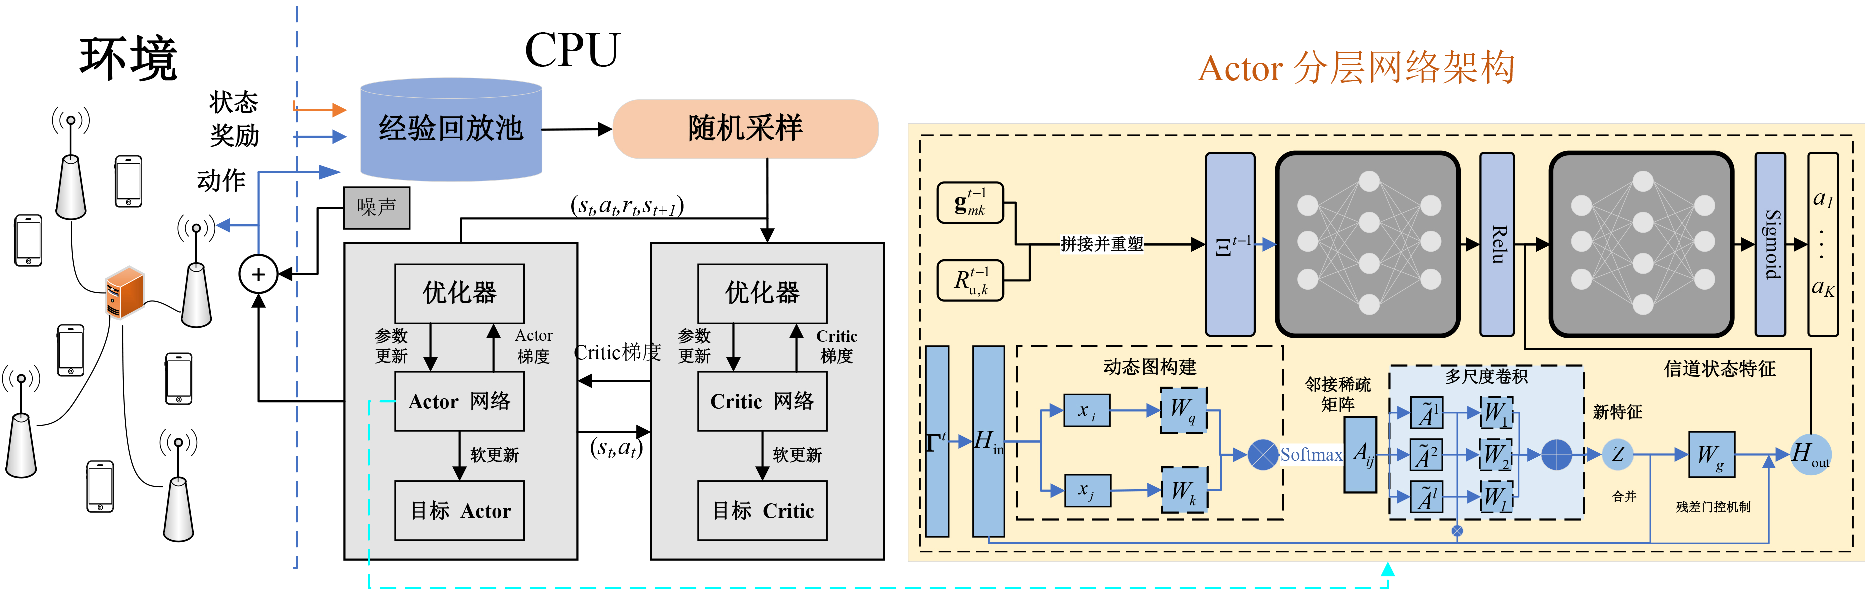
\includegraphics[width=5in] {fig2}
\caption{DMAGNN-AC网络架构图。}
\label{fig2}
\end{figure}

\subsection{DMAGNN-AC 组件}
$\emph{1) 状态}$：本文在第三节中指出，第 \(k\) 个用户设备与第 \(m\) 个接入点之间的信道状态信息 \(\mathbf{g}_{mk}\) 到第 \(k\) 个用户设备功率控制系数 \(\eta_k\) 之间存在某种映射函数。但由于中央处理单元（CPU）无法获取信道实时观测值，本文最终采用理论信道状态信息 \(\mathbf{g}_{mk}\) 作为神经网络的输入。因此，神经网络的输入可表示为
\begin{equation}\mathbf{\Gamma}^t:=\left \{  \mathbf{g}_{mk}^t  \mid \forall m,k\right \}.	\end{equation} 

然而，考虑到训练过程本质上是与时间序列紧密相关的马尔可夫过程，直接将变量 $\mathbf{\Gamma}^t$ 作为神经网络的输入并不合理。同时，在指定时间跨度内，用户移动行为引发的环境状态变化可被视为一个时间序列演化过程；在该演化过程中，用户在时空维度的移动特征是预测其下一时刻行为的关键依据。

为此，本文引入时刻 $(t-1)$ 下的 $\mathbf{g}_{mk}$ 与 $R_{\text{u},k}$ 作为神经网络输入的辅助信息，使其与 $\mathbf{\Gamma}^t$ 共同参与下一时刻动作的预测。辅助信息的具体定义为
\begin{equation}\mathbf{\Xi} ^{t-1}:=\left \{\mathbf{g}_{mk}^{t-1} , R_{\text{u},k}^{t-1} \mid \forall m,k \right \}  .\end{equation} 
神经网络的最终输入可表示为
\begin{equation}s^{t}:=\left \{ \mathbf{\Xi} ^{t-1}, \mathbf{\Gamma} ^t\right \}. \end{equation}
此时，状态空间的基数为$2 \left ( MK \right ) +K$。

$\emph{2) 动作}$：演员网络根据当前状态 \(s\) 进行决策，输出 \(K\) 个用户设备的上行发射功率系数，可表示为
\begin{equation}a ^{t}=\left [ \eta _1^{t},...,\eta _K^{t} \right ] ,\end{equation}

式中，$\eta _k^{t}$满足约束条件 $0\le \eta _k^{t}\le \eta _\text{max}, \forall k$。

\emph{3) 奖励}：本文直接以实际获得的用户速率作为环境反馈的奖励函数，其定义为
\begin{equation}r^{t+1} = \textstyle \sum_{k=1}^{K} R_{\text{u},k}^{t}.\end{equation}

\subsection{算法设计}
所提算法的具体设计体现在以下四个方面。
\subsubsection{Actor 网络分层设计}
本文将 Actor 网络设计为分层结构，旨在合理划分功能并有效融合信息。具体而言，上层网络主要对信息 $\mathbf{\Xi }^{t-1}$ 进行特征提取与融合；随后，将上层网络的输出与信息 $\mathbf{\Gamma} ^t$ 的特征相结合，作为下层网络的输入。下层网络的核心功能是基于上述融合特征完成动作预测。

在将 $\mathbf{\Gamma} ^t$ 输入至下层网络之前，本文采用自主设计的DMAGNN对 $\mathbf{\Gamma} ^t$ 进行特征提取。DMAGNN的运行流程包含以下步骤：
\begin{itemize}
\item {\bf{节点特征初始化：}}
第 \(k\) 个用户设备在 \(t\) 时刻的节点特征被初始化为
\begin{equation}\label{eq-38}x_k=\text{vec}(H_{\text{in},k}^HH_{\text{in},k})\in \mathbb{R}^d, \end{equation}
式中，$H_{\text{in},k}\in \mathbb{C} ^{M\times N}$ 表示第 \(k\) 个用户设备到 \(M\) 个接入点（AP）的信道矩阵。

\item{\bf{动态图结构学习}}
在图构建过程中，传统图结构通常依靠固定的地理距离（如路径损耗）来定义节点间的连接关系。然而在CF‑mMIMO系统中，用户设备分布密集、干扰特性复杂，固定图结构无法反映瞬时信道状态带来的影响。为此，本文借鉴图注意力网络（GAT）的注意力机制，引入可学习的参数化距离度量，并利用双线性注意力机制计算节点 \(i\) 与节点 \(j\) 之间的关联强度。
\begin{equation}\label{eq-39}a_{ij}=\sigma \left ( \frac{\left ( W_qx_i \right ) \cdot \left ( W_kx_j \right )  ^T}{\sqrt{b} } \right  ), \end{equation}
式中，$b$ 为缩放因子，$W_q$ 和 $W_k$ 是可训练的投影矩阵，用于将节点特征 $x_i$、$x_j$ 分别映射到查询空间与键空间。
查询空间用于表示当前节点（如用户 $i$）的查询特征，键空间则用于表示其他节点（如用户 $j$）的被查询特征。
通过计算二者的内积，可以衡量两个节点之间的关联程度与相似度。该机制使模型能够动态学习节点间的关联关系，而非依赖预先定义的图结构。

{\emph{定理 2:}} 为降低全连接图 $O(K^2)$ 的计算复杂度，本文设计了稀疏邻接矩阵形式。
\begin{equation}\label{eq-40}A_{ij}=\left\{\begin{matrix}
  1,& \text{if} \hspace{0.1cm} a_{ij}> \vartheta \hspace{0.1cm} \text{and}\hspace{0.1cm} i\ne j\\ 
  0,& \text{otherwise},
\end{matrix}\right.\end{equation}
式中，动态阈值 $\vartheta$ 通过自适应二分搜索确定，以保证非零边的数量满足 $\left | E \right | =O\left ( K\log K \right )$。
通过对邻接矩阵进行稀疏化处理，模型仅保留相关性较强的连接，从而提升泛化性能。

\item{\bf{多尺度特征聚合：}}
多尺度卷积通过聚合不同范围的邻域信息，增强模型对复杂空间相关性的捕获能力，从而解决传统单层图卷积网络（GCN）感受野有限的问题。多跳信息聚合公式可表示为
\begin{equation}\label{eq-41}\text{GCN}\left ( A,H_{\text{in}} \right ) =\sum_{l=0}^{L} \tilde{A} ^lH_{\text{in}}W_l,\end{equation}
式中，$\tilde{A} =D^{-\frac{1}{2}}AD^{-\frac{1}{2}}$ 为邻接矩阵 $A$ 的对称归一化形式，$D=\text{diag}\left(\sum_j A_{1j},\dots,\sum_j A_{Kj}\right)$ 为度矩阵，$W_l\in\mathbb{R}^{d\times d}$ 为第 $l$ 跳对应的可训练权重矩阵。该设计具备以下特点：
\begin{itemize}
    \item 局部性保持：当 \(l=0\) 时，保留节点自身特征。
    \item 邻域扩展：$l=1$ 时聚合一阶邻域信息，$l=2$ 时捕获二阶邻域信息。
\end{itemize}
同时，为不同跳数设置独立的 $W_l$，以避免特征混淆。

\item{\bf{门控特征更新机制：}}
最后，本文采用门控机制实现节点特征的选择性更新，具体过程可表示为
\begin{equation}\label{eq-42}Z=\text{GCN}\left ( A,H_{\text{in}} \right ), \end{equation}
\begin{equation}\label{eq-43}G=\sigma \left ( W_g\left [ H_{\text{in}}  \oplus Z \right ]  \right ),\end{equation}
\begin{equation}\label{eq-44}H_{\text{out}}=\text{LayerNorm}\left ( G\odot H_{\text{in}}+\left ( 1-G \right ) \odot Z \right ), \end{equation}
式中，$Z$ 为卷积后生成的新特征，$W_g\in\mathbb{R}^{2d\times d}$ 为门控权重矩阵。
门控机制可动态选择保留原始特征 $H_{\text{in}}$ 与新特征 $Z$ 的比例，从而缓解梯度消失问题。
\end{itemize}

\begin{algorithm}[t]
    \renewcommand{\algorithmicrequire}{\textbf{输入:}}
    \renewcommand{\algorithmicensure}{\textbf{输出:}}
    \caption{DMAGNN-AC 功率分配算法}
    \label{DDPG}
    \begin{algorithmic}[1]
    			\State $\emph{输入：}$ 回合次数 $T_e$， 探索次数 $T$， 折扣因子 $\gamma$， 学习率 $\alpha$， 随机数据量 $R_q$， 批次大小 $\mathcal{N}$， 神经网络更新权重 $\tau$。 % input
    			
    			\State $\emph{初始化：}$ 采用 He 初始化方法\footnotemark[1]初始化Critic网络 $C(s,a;\omega _c)$、Actor网络 $A(s;\omega _a)$ 的参数 $\omega _c$ 和 $\omega _a$，并且初始化 DMAGNN 的参数与初始状态 $s^1$。

        \For {$k=1$ to $T_e$}
        		\State 设置环境变量初始值。
        		
	        \For {$\jmath =1$ to $T$}
	        		\State 二分搜索阈值 $\vartheta$.
	            
		        \If {$\jmath < R_q$}
		            \State 以均匀概率随机生成动作 $a^t$。 
		        \Else
		        	  \State 由式 \eqref{eq-38}--\eqref{eq-40} 构建动态图。
		        	  \State 根据式 \eqref{eq-41} 进行多尺度特征聚合。
		        	  \State 根据式 \eqref{eq-42} 执行门控特征更新，并输出新的特征向量 $H_{\text{out}}$。
		            \State 根据式 \eqref{eqn-34} 选择动作 $a^t$。
		        \EndIf
		        \State 执行动作 $a^t$，获得奖励 $r^t$ 与下一状态 $s^{t+1}$。
		        \State 存储该交互样本$(s^{t},a^{t},r^{t},s^{t+1})$。
		        \State 根据式 \eqref{eqn-38} 计算Critic网络梯度 $\nabla \omega _c$，并沿负梯度方向更新 $\omega _c$：$\omega _c\longleftarrow \omega _c-\alpha \nabla \omega _c$。
		        \State 根据式 \eqref{eqn-37} 计算Actor网络梯度 $\nabla \omega _a$，并沿正梯度方向更新 $\omega _a$：$\omega _a\longleftarrow \omega _a+\alpha \nabla \omega _a$。
		        \State 将目标评论家网络权重与目标行动者网络权重更新为：
		        \State \hspace{6mm}$\omega  _c^{'}\longleftarrow \tau \omega  _c+(1-\tau )\omega  _c^{'}$.
		        \State \hspace{6mm}$\omega  _a^{'}\longleftarrow \tau \omega  _a+(1-\tau )\omega  _a^{'}$.
	        \EndFor
        \EndFor
        \State $\emph{输出:}$每个数据集可达到的最大用户速率 $R_{\text{u},k}$。 % output
		\end{algorithmic}
\end{algorithm}

\footnotetext[1]{He 初始化是深度学习中一种神经网络权重初始化方法，该方法基于 ReLU 激活函数的特性，用于提升训练过程中的收敛速度与网络性能。}

这种分层设计的优势在于，上层网络能够充分挖掘前一时刻信息中的关键特征，为下层网络提供更具价值的先验信息。因此，下层网络在预测动作时，可以更精确地基于时刻 $t$ 的信息进行决策。该设计提升了整体网络的学习效果与决策精度。

\subsubsection{网络更新频率的优化策略}
为进一步优化网络学习过程，本文设计了一种目标网络更新频率（UF）的动态调整策略。在每轮完整训练开始时，首先将目标网络更新频率初始化为 $300$，并将初始最大奖励（MR）设为 $0$。随着训练推进，持续计算奖励值的累积结果。当训练步数达到设定的更新频率时，计算当前阶段的平均奖励（AR）并与最大奖励（MR）进行比较。若平均奖励超过最大奖励，则将最大奖励更新为当前平均奖励，并根据最大奖励与平均奖励之间的差值 $D_\text{value}$ 构建网络更新频率调整公式，具体如下所示。
\begin{equation}\text{UF}=\text{UF}\times \log_{2}{\left ( 1+\frac{1}{1+e^{D_\text{value}} }  \right ) }. \end{equation}

该公式表明：当 $D_{\text{value}}$ 更新幅度较大时，网络表现出更优的学习性能，此时加快目标网络的更新频率，可使网络更及时地追踪最优策略。反之，若 $D_{\text{value}}$ 更新跨度较小，则降低更新频率，避免因更新过快导致网络不稳定或陷入局部最优。

\subsubsection{训练回滚策略}
此外，当平均奖励（AR）小于最大奖励（MR）时，将网络状态重置为本轮训练开始时的状态并重新训练。该策略有助于网络跳出可能存在的局部最优解，重新探索更优策略空间，提升整体学习成功率与效率。

\subsubsection{训练过程}
如图 \ref{fig2} 所示，DMAGNN-AC 框架由两个主要网络构成：行动者网络与评论家网络。智能体借助行动者网络 $A(s;\omega_a)$，根据当前状态 $s$ 生成确定性动作 $a$，其中 $\mathbf{\omega}_a$ 为行动者神经网络的参数。评论家网络 $C(s_c,a;\omega_c)$ 对基于当前状态 $s_c$ 所选择的动作进行评估。该确定性策略可表示为
\begin{equation}a ^* = A(s;\omega  _a).\end{equation}
同时，本文引入高斯噪声以提升模型泛化能力，具体表达式如下。
\begin{equation}\label{eqn-34}
a := \left [ A(s;\omega  _a)+\mathbf{n} \right   ]^{P_\text{max}}_0 ,
\end{equation}
其中 $\mathbf{n}\sim \mathcal{CN}(0,1)$。动作 $a$ 的取值区间为 $\left [ 0,P_\text{max} \right ] $。
为获得最大奖励，行动者网络与评论家网络协同调整行动者网络参数，以最大化评论家网络的输出。其公式可表示为
\begin{equation}\omega  _a^* = \underset{\omega  _a}{\text{argmax}} C(s_c,a;\omega  _a).\end{equation}
此外，评论家网络通过不断调整参数，减小预测值与实际奖励之间的误差，以提升预测精度。其数学表达式为
\begin{equation}\omega  _c^* = \underset{\omega  _c}{\text{argmin}}\frac{1}{2} ( C(s_c,a;\omega  _c)|_{a=A(s;\omega  _a)}-r_s^a)^2.\end{equation}

行动者网络通过最小化行动者梯度来更新参数，其表达式为
\begin{equation}\label{eqn-37}\nabla  _{\omega_a} J(\omega_a)\approx \frac{1}{T} \sum_{t=1}^{}\nabla  _aC(s^t,a^t;\omega _c)
\nabla  _{\omega _a}A(s^t;\omega _a). \end{equation}
对于评论家网络而言，其可通过如下损失函数更新参数
\begin{equation}\label{eqn-38}\nabla _{\omega _c}L(\omega _c) \approx \frac{1}{T} \sum_{t=1}^{} (y^t -C(s^t,a^t;\omega _c))^2,\end{equation}
其中 $y^t=r^t+\gamma C\left ( s^{t+1},a^{t+1};\omega _c'\right )$，$\gamma$ 为折扣因子。
该算法的具体实现过程详见上页顶部的算法 \ref{DDPG}。

\begin{figure}
\centering
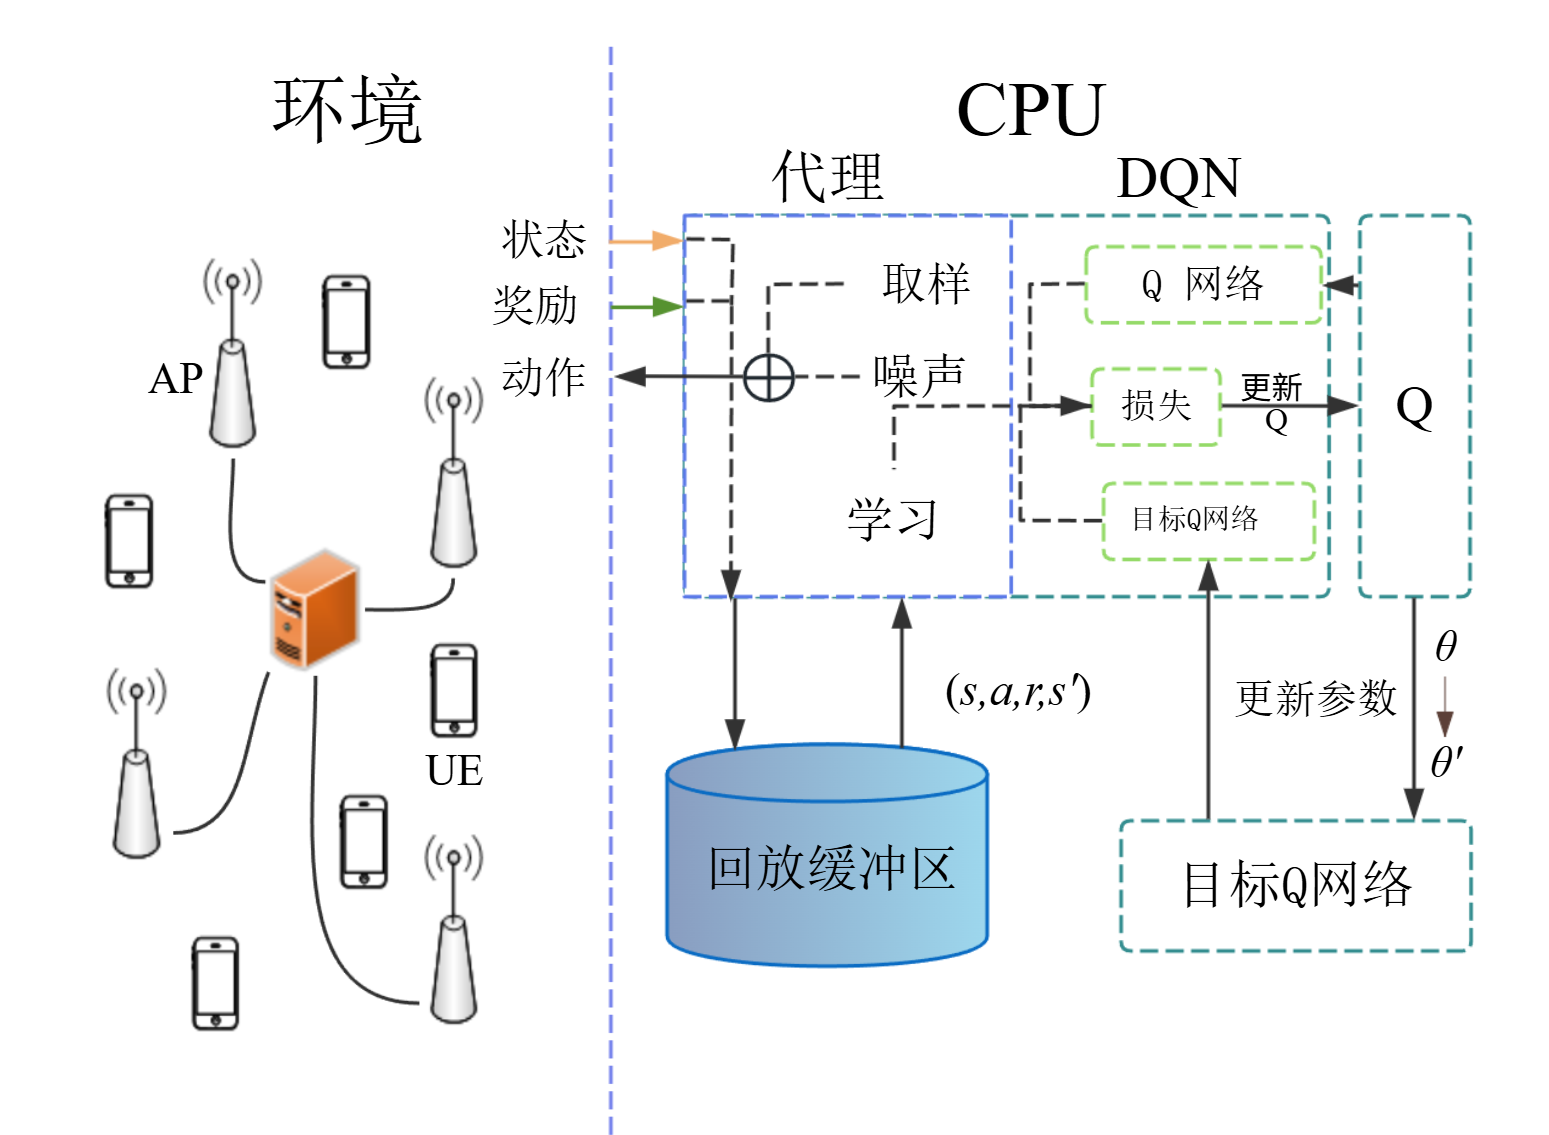
\includegraphics[width=3.5in] {fig3}
\caption{Network architecture of MADQIN.}
\label{fig3}
\end{figure}

\renewcommand{\thefootnote}{\ding{\numexpr192+\value{footnote}}}
\begin{algorithm}[t]
    \renewcommand{\algorithmicrequire}{\textbf{Input:}}
    \renewcommand{\algorithmicensure}{\textbf{Output:}}
    \caption{MADQIN Algorithm}
    \label{DQN}
    \begin{algorithmic}[1]
        \State $\emph{Input:}$ Episode times $N_e$, exploration times $T$, target network update frequency $T_u$, discount factor $\gamma$, learning rate $\alpha$, and random data quantity $R_q$. % input
      	  \State $\emph{Initialization:}$ Initialize MADQIN $Q(s,a;\omega _q)$ parameter $\omega _q$ with He initialization method.
    			% for loop
        \For {$k=1$ to $N_e$}
        		\State Creating environment object $  \mathcal{O} _e$ and neural network object $  \mathcal{O} _d$.
        		\State Initialize status $s^1$.
        		% for loop
	        \For {$ \jmath  =1$ to $T$}
	            % if ... else
		        \If {$ \jmath  < R_q$}
		            \State Randomly select action set $a^t\in \mathcal{A}$ with uniform probablity. 
		        \Else
		            \State Select action $a^t$ by \eqref{eqn-39}.
		        \EndIf
		        \State Execute action $a^t$, obtain reward $r^t$, and next state $s^{t+1}$.
		        \State Store the transaction$(s^{t},a^{t},r^{t},s^{t+1})$.
		        \State Minimizing the loss to update the MADQIN network.
		        \State \begin{align} L^t(\omega _q^t)&= (r_{s,a}^t+\gamma \underset{a^{t+1}}{\text{max}}Q(s^{t+1},a^{t+1};\omega_{target})
		        					\nonumber\\&\quad-Q(s^t,a^t;\omega_q ^t) )^2. \nonumber\end{align}
	        \EndFor
        \EndFor
        \State $\emph{Output:}$ Learned DQN $Q(s,a;\omega _q)$. % output
        
		\end{algorithmic}
\end{algorithm}

\section{MADQIN算法设计}

考虑到模数转换器（ADC）分辨率的离散特性，本章采用离散动作空间的深度Q网络（DQN）作为优化框架，并设计了一种离散动作空间的多智能体深度Q集成网络（MADQIN）。如图 \ref{fig3} 所示，该算法架构主要由Q网络（Q-Network）和目标Q网络（Q-target）两个神经网络构成。MADQIN通过Q网络预测系统内智能体动作的最大Q值，并将其作为预测奖励 $r_p$；随后智能体选择Q值最高的动作执行，以获取实际奖励 $r$。此外，目标Q网络用于预测下一状态的Q值 $r_t$，并将 $r$ 与 $r_t$ 之和作为真实奖励 $r'$。通过迭代不断更新Q网络的参数 $\omega_q$，以最小化 $r_p$ 与 $r'$ 之间的误差。该优化目标的具体表达式为
\begin{equation}\omega  _q^* = \underset{\omega  _q}{\text{argmin}} \frac{1}{2} (Q(s ,a ;\mathbf{\omega  } _q)-r_s^a)^2.\end{equation}
$\omega_q$ 的梯度计算方法为：
\begin{equation}\nabla \omega _q = (Q(s,a;\omega _q)-r_s^a)\nabla _{\omega _q}Q(s,a;\omega _q).\end{equation}

在深度强化学习（DRL）环境中，本文将MADQIN的输出层维度定义为 $[M, AD]$，其中 $AD$ 表示每个接入点（AP）可采用的ADC分辨率可选数量。该网络的输出旨在预测 $M$ 个AP在给定状态集合下执行每一种可能动作对应的Q值。为选取最优动作策略，本文求解使Q值最大化的动作 $a^*$。该策略通过融合 $M$ 个深度Q网络（DQN）的预测结果实现，确保在多AP环境下选中最优的ADC分辨率配置。最优动作集合可通过如下公式求得，
\begin{equation}\label{eqn-39}a^* = \underset{a}{\text{argmax}}Q(s,a;\omega  _q).\end{equation}

MADQIN网络的输入与输出设计与DMAGNN-AC的组件设计保持一致。不同于传统方法中通过贪心策略最大化样本多样性的思路，本文选择在初始 $\jmath$ 步采用随机动作策略，并将这些动作产生的数据纳入经验回放缓冲区。该方式提升了模型的鲁棒性与适应性。通过一系列实验验证，本文证明该随机动作策略在研究的特定场景下表现出更优效果。此外，为进一步提升算法性能，本文在执行动作时引入高斯随机噪声，其表达式为
\begin{equation}a := \left [ a^*+\mathbf{n} \right   ]^{b_m^\text{max}}_{b_m^\text{min}} .\end{equation}

\begin{table}[t]
  \begin{center}\label{table1}
    \caption{System basic parameter settings.}
    \begin{tabular}{@{}lll@{}}
			\toprule
                          & \textbf{Parameters}                        & \textbf{Values} \\ \midrule
 							    				 & Carrier frequency                   	& 1.9 GHz             \\
                          & Bandwidth                    				 	& 20 MHz          \\
                          & Noise figure           & 9 dB   \\
                          & AP antenna height & 15 m     \\
                          & User antenna height   & 1.65 m           \\
                          & Coherence interval length $\tau$        & 200\\
                          & Pilot length $\tau_\text{p}$   & 20  \\
                          & Pilot transmission power $\rho_\text{p}$              & 200 mW             \\
                          & ADC resolution $b_m$            &10   \\
                          & $M$, $K$, $N$    & 100, 20, 4\\
                          &$\delta _\text{sh}$, $L$, $d_1$, $d_0$   & 8 dB, 140.7 dB, 50 m, 10 m     \\\midrule
			\end{tabular}
  \end{center}
\end{table}

\begin{table}[t]
  \begin{center}\label{table2}
    \caption{Neural Network Parameter Settings.}
    \begin{tabular}{@{}lll@{}}
			\toprule
			                          & \textbf{Parameters}                        & \textbf{Values} \\ \midrule
			\multirow{6}{*}{DMAGNN-AC} & Discount factor $\gamma$                   & 0.1             \\
			                          & Learning rate $\alpha $                    & 0.001           \\
			                          & Size of experience replay buffer $\mathcal{B}$           & 10000   \\
			                          & Frequency of updating initial trial status $\mathcal{H}$ & 500     \\
			                          & Update neural network parameter weights $\tau$   & 0.005           \\
			                          & Warm up times   $\mathcal{W}$              & 256             \\ \midrule
			\multirow{5}{*}{MADQIN}   & Learning rate   $\alpha $                  & 0.001           \\
			                          & Discount factor $\gamma$                   & 0.1             \\
			                          & Size of experience replay buffer  $\mathcal{B}$         & 1000     \\
			                          & Batch size      $\varsigma$                & 200             \\
			                          & Warm up times  $\mathcal{W}$               & 200             \\ \midrule
			\end{tabular}
  \end{center}
\end{table}
MADQIN的详细执行流程总结于本页顶部的算法 \ref{DQN} 中。

\section{数值结果与分析}
在本节中，本文通过一系列实验结果，对搭载非线性功率放大器（PA）与低分辨率模数转换器（ADC）的CF‑mMIMO系统性能进行阐述与分析。如无特殊说明，均采用表Ⅰ所示的标准实验参数配置。

本文在研究中沿用文献 \cite{paper15} 中非线性PA模型的系数设置，其中 $a_1=13.85$，$a_3=-4.074$。对于大尺度衰落系数模型 $\beta_{mk}$，本文采用特定建模方式，以精准反映实际通信环境中的信号衰减特性。

\begin{equation}\beta _{mk} = \text{PL}_{mk}\cdot 10^{\frac{\delta _{\text{sh}^zmk}}{10} },\end{equation}
其中 $10^{\frac{\delta_{\text{sh}^zmk}}{10}}$ 用于模拟阴影效应，$z_{mk}\sim \mathcal{CN}(0,1)$。变量 $\text{PL}_{mk}$ 表示路径损耗，遵循文献 \cite{paperI4} 提出的三斜率模型。路径损耗（单位：dB）为
\begin{equation}\text{PL}_{m k}=\left\{\begin{array}{l}
-L-35 \log _{10}\left(d_{m k}\right), \text { if } d_1<d_{mk} \\
-L-15 \log _{10}\left(d_{1}\right)-20 \log _{10}\left(d_{m k}\right), \\
\quad\quad\quad\quad\quad\quad\quad\quad\quad\quad\quad\text { if } d_{0}<d_{m k} \leq d_{1} \\
-L-15 \log _{10}\left(d_{1}\right)-20 \log _{10}\left(d_{0}\right), \text { if } d_{m k} \leq d_{0}
\end{array}\right.\end{equation}

需要注意的是，当 $d_{mk}<d_{1}$ 时不存在阴影效应。

为验证所提算法的性能，本文将其与基础的全功率发射方法进行对比。大量实验结果表明，在每种环境下约 2000 步即可达到理想效果。两种算法的相关参数总结于表Ⅱ中。

\begin{figure}
\centering
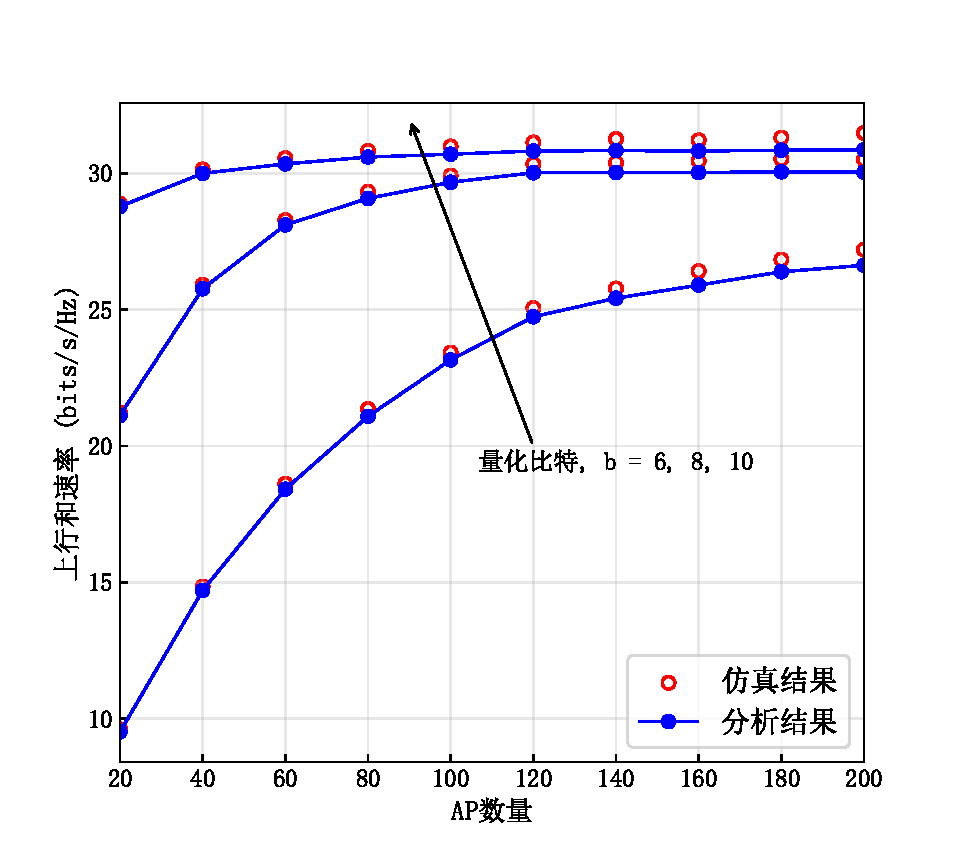
\includegraphics[width=3.2in] {MonteCarlo}
\caption{Achievable uplink sum-rate versus the number of APs, with $K=20$, $N=20$.}
\label{MonteCarlo}
\end{figure}

首先，图 \ref{MonteCarlo} 给出了上行可达和速率与接入点（AP）数量之间的关系。此外，本文对式 \eqref{eqn-23} 对应的“解析结果”与式 \eqref{eqn-22} 给出的“仿真结果”进行了对比分析。“仿真结果”通过蒙特卡洛方法，在 $10^4$ 次独立同分布（i.i.d.）信道实现下完成验证。可以清晰地看出，“仿真结果”与“解析结果”高度吻合，充分证明了推导结果的准确性，为后续相关理论研究奠定了坚实基础。

\begin{figure}
\centering
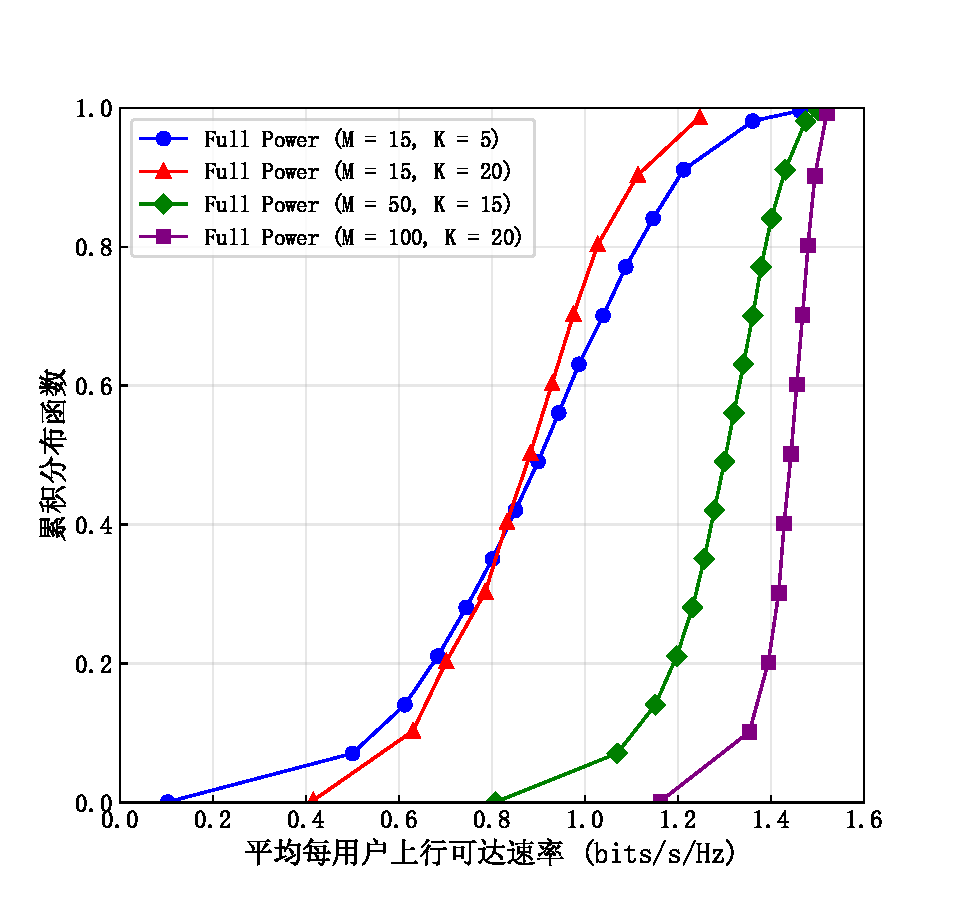
\includegraphics[width=3.2in] {fig4}
\caption{Uplink per-user rate under different numbers of APs and UEs during full power transmission, with $N$ = 4, $b_m$ = 10.}
\label{fig4}
\end{figure}


图 \ref{fig4} 给出了全功率传输时，不同接入点（AP）与用户设备（UE）数量下单用户速率的累积分布函数（CDF）曲线。可以看出，当 $M=15$ 时，随着UE数量增加，平均单用户速率呈下降趋势。这是因为随着UE密度升高，导频污染与多用户干扰愈发严重。值得注意的是，尽管平均速率有所下降，用户速率下界却有所提升。主要原因是：当AP数量远大于UE数量时，系统尚未达到最大服务容量。而当UE数量超过AP数量时，用户速率会受到明显干扰，这一问题可通过增加AP数量来缓解。随着UE与AP数量增加，CDF曲线逐渐右移，并最终收敛于共同上限值 $1.5$ bits/s/Hz。结果表明：在本文研究场景中，单纯增加AP与UE数量并不能无限制提升用户速率，但可以提高用户速率下界，增强系统数据传输的稳定性。
这体现了CF‑mMIMO系统的特点：能够为所有用户提供稳定、均匀的服务质量。

\begin{figure}
\centering
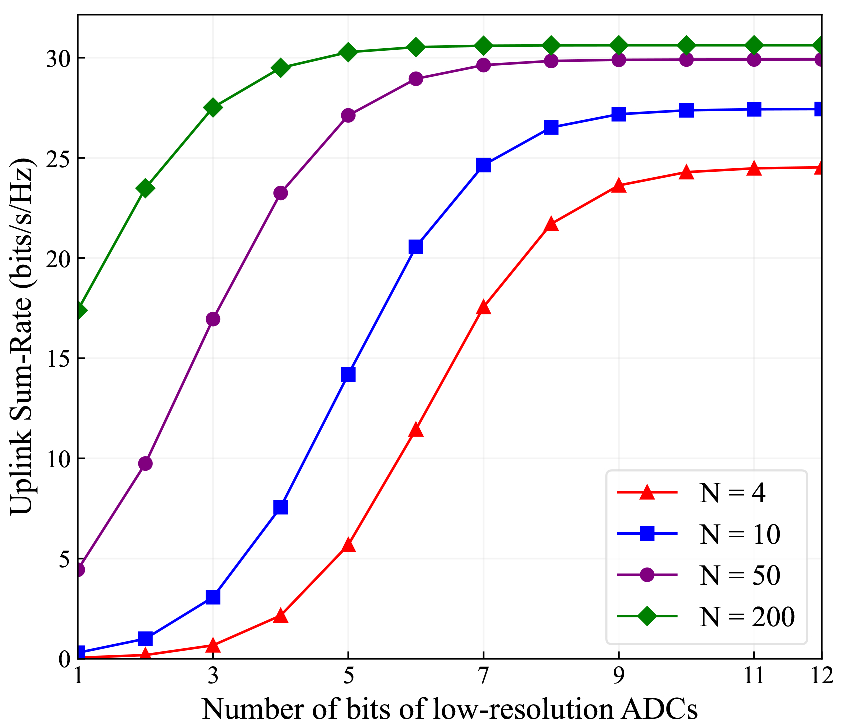
\includegraphics[width=3.2in] {fig5}
\caption{The relationship between uplink sum-rate and the number of bits of low resolution ADCs under different numbers of AP antennas, with $M$ = 100, $K$ = 20.}
\label{fig5}
\end{figure}
\begin{figure}
\centering
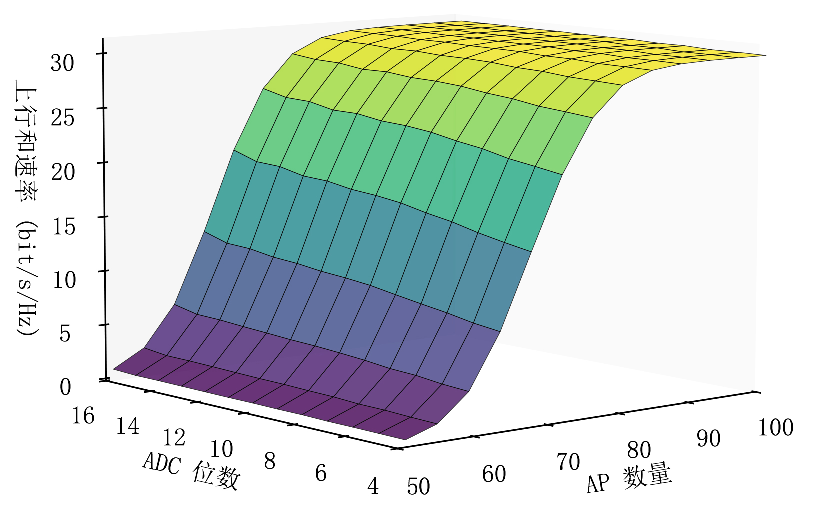
\includegraphics[width=3.5in] {fig6}
\caption{The impact of ADC bit count and AP count on uplink sum-rate, with $K$ = 20.}
\label{fig6}
\end{figure}

图 \ref{fig5} 和图 \ref{fig6} 分别展示了在多种影响因素存在时，低分辨率ADC的比特位数对上行用户和速率的影响。在每组实验中，假设所有AP配备相同分辨率的ADC。
从两幅图中均可明显看出：在达到峰值速率之前，提高ADC分辨率能够显著提升用户速率。但在更大尺度下，AP数量成为决定用户速率的主要因素，这表明增加AP数量可以补偿由低分辨率ADC带来的速率损失。此外，天线数量不足会导致系统无法达到用户速率的最大潜在性能。如图 \ref{fig5} 所示，仅当 $N \ge 50$ 时用户速率才接近极限，这说明在实际部署中，需根据AP数量合理配置天线数量，才能充分发挥系统性能。同时，随着天线数量增加，单用户速率逐渐趋于上限 $1.5$ bits/s/Hz，与前文结论一致。当 $N$ 相对于
${\rho _\text{u}}\sum\limits_{m = 1}^M {\alpha _m}(1 - {\alpha _m})\left( \sum\limits_{k = 1}^K {\beta _{mk}}\Omega _k + 1 \right){\gamma _{mk}}$
足够大时，其对用户速率的影响逐渐减弱。此外，图 \ref{fig5} 与图 \ref{fig6} 中的峰值速率基本一致，表明单纯提升ADC分辨率与AP天线数量无法突破系统固有的速率上限。

\begin{figure}
\centering
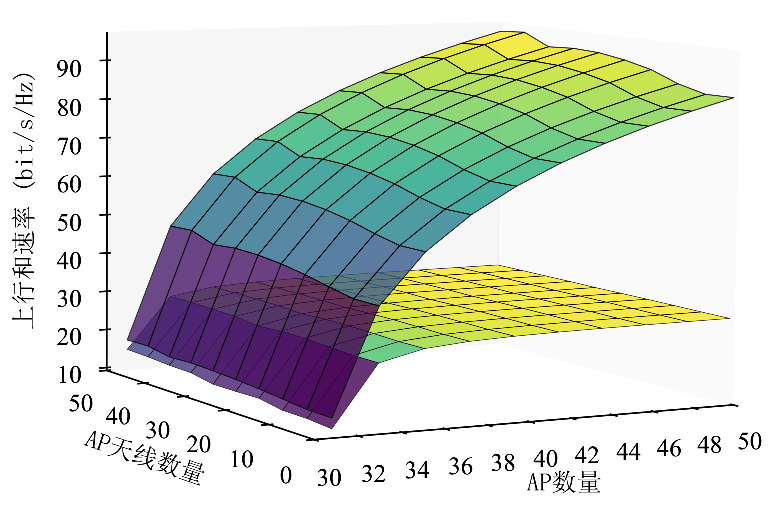
\includegraphics[width=3.5in] {fig7}
\caption{Comparing the uplink sum-rate in a CF-mMIMO system with nonlinear PAs and low-resolution ADCs versus the ideal hardware scenario, with $b_m$ = 10.}
\label{fig7}
\end{figure}

随后，本文对比分析了理想硬件条件与非理想硬件条件下，CF‑mMIMO系统在不同AP数量与AP天线数量时的可达用户速率。如图 \ref{fig7} 所示，在理想硬件条件下，随着AP数量与天线数量的增加，用户和速率最高可超过 90 bits/s/Hz。然而，受非线性PA**与低分辨率ADC的影响，用户和速率的峰值被限制在 30 bits/s/Hz 左右。结果表明，硬件损伤的存在使系统速率下降近 70\%，这凸显了对含硬件损伤系统开展深入研究的必要性。
\begin{figure}
\centering
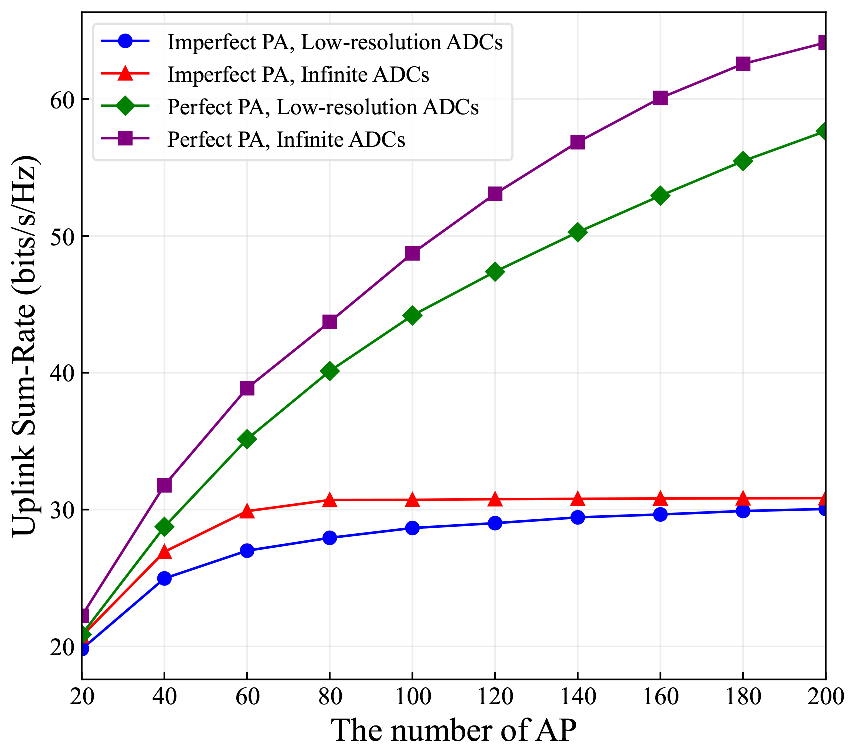
\includegraphics[width=3.2in] {compare}
\caption{Rate comparison based on different hardware impairments, with $b_m$ = 10, $K$ = 20.}
\label{compare}
\end{figure}

随后，为深入分析导致用户速率显著下降的主要因素，图 \ref{compare} 通过控制硬件损伤变量设计了对比实验。实验结果表明，在假设ADC具有无限分辨率的理想条件下，PA的非线性成为限制用户速率上限的关键因素，这有力支撑了我们对式 \eqref{eqn-23} 的分析结论。

\begin{figure}
\centering
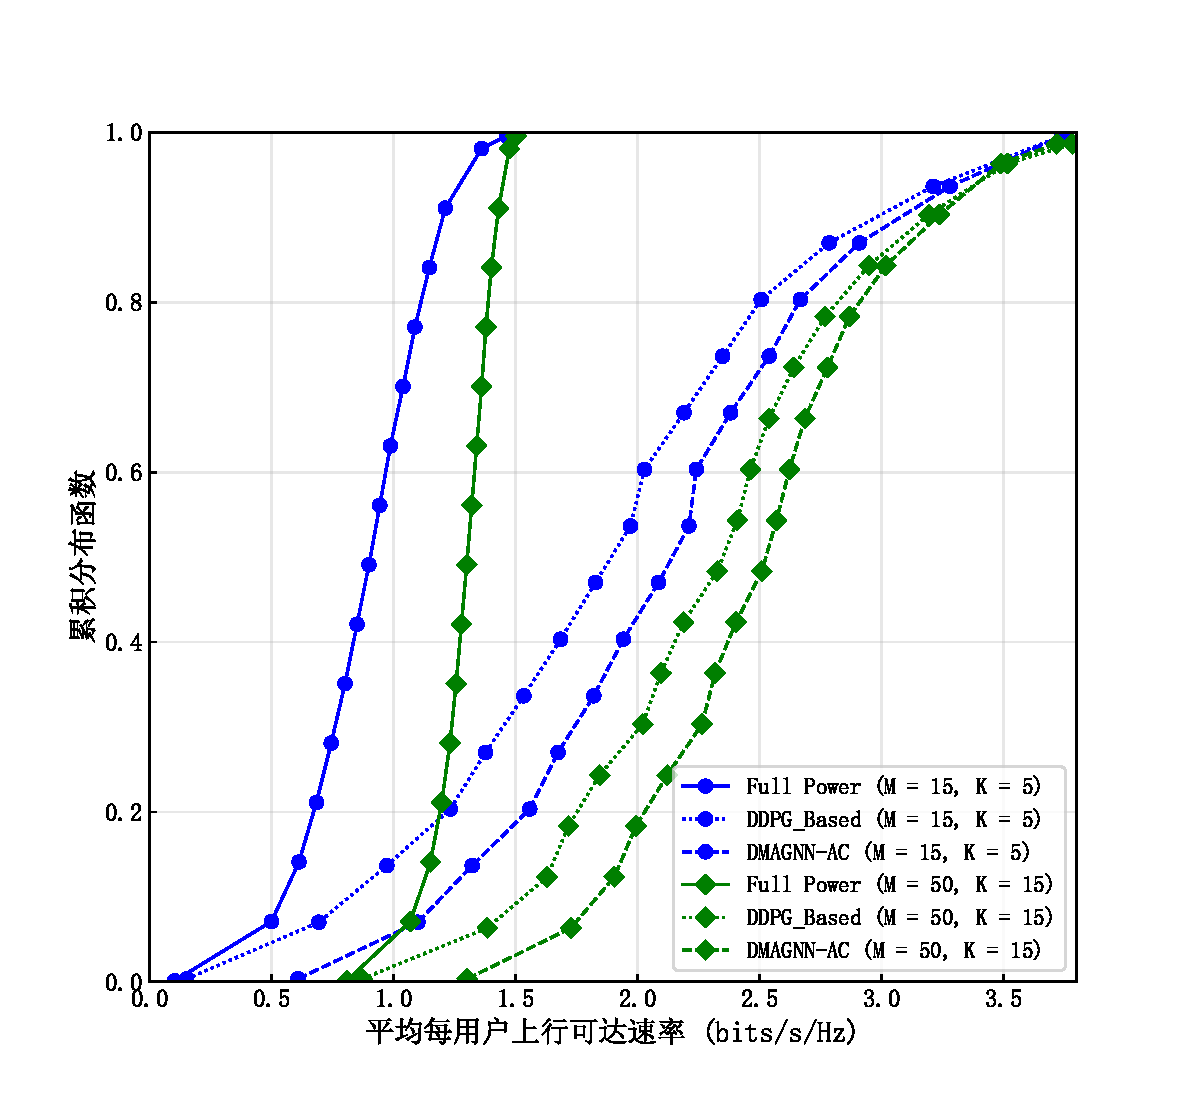
\includegraphics[width=3.2in] {fig10}
\caption{Comparison of per-user rate between full power transmission, DDPG$\_$Based, and DMAGNN-AC algorithm, with $b_m$ = 10, $N$ = 4.}
\label{fig10}
\end{figure}
\begin{figure}
\centering
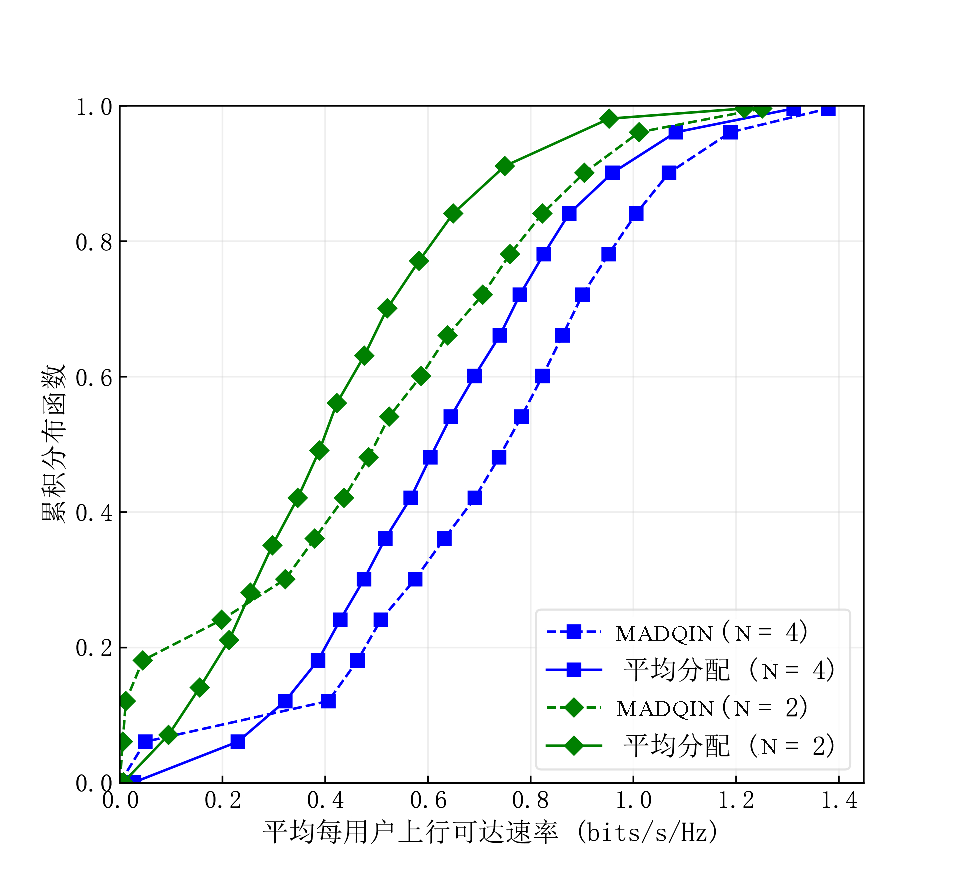
\includegraphics[width=3.2in] {fig11}
\caption{Comparison of average allocation and the MADQIN algorithm under the same total bit count, with $b_\text{total}$ =135, $M$ = 15, and $K$ = 5.}
\label{fig11}
\end{figure}

接下来，本文利用所提算法对整个系统中各AP与UE的实验参数进行精细调控，从不同角度验证算法带来的性能提升。图 \ref{fig10} 对比了DMAGNN‑AC算法与全功率传输策略、DDPG算法的优化性能。DDPG算法通过与环境交互探索逐步逼近最优解，在达到全功率策略性能上限后，可将单用户速率进一步提升 $2.8$ bit/s/Hz。此外，在引入DMAGNN作为特征提取模块后，速率的累积分布曲线相对DDPG进一步右移，验证了DMAGNN通过干扰建模与多尺度特征融合，能够提升算法收敛性能并改善最小用户速率。不同AP‑UE配置下的对比结果表明，系统最高用户速率稳定在 $3.8$ bit/s/Hz 左右，即为用户速率的最终性能边界。

如图 \ref{fig11} 所示，在总比特数保持恒定的前提下，本文所提的MADQIN算法相比平均分配策略在性能上有显著提升。随着天线数量增加，用户速率呈逐步上升趋势。值得注意的是，调整AP的ADC分辨率仅能带来较小的性能增益。这一现象可由式 \eqref{eqn-23} 解释：速率主要由ADC总分辨率决定，无论信号是期望信号还是用户间干扰，仅有ADC量化噪声项与分辨率的具体分配有关。因此，该影响处于可接受范围内。

\begin{figure}
\centering
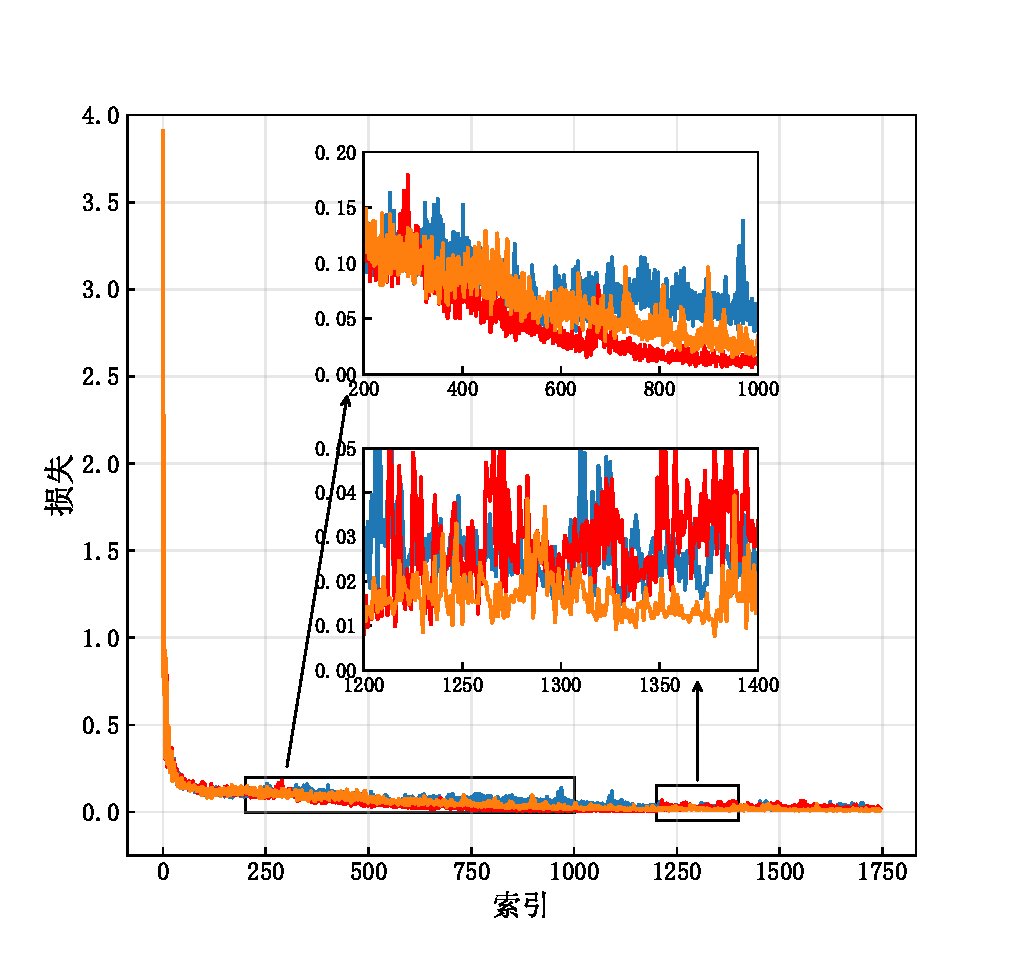
\includegraphics[width=3.2in] {fig8}
\caption{Convergence of DMAGNN-AC algorithm.}
\label{fig8}
\end{figure}
\begin{figure}
\centering
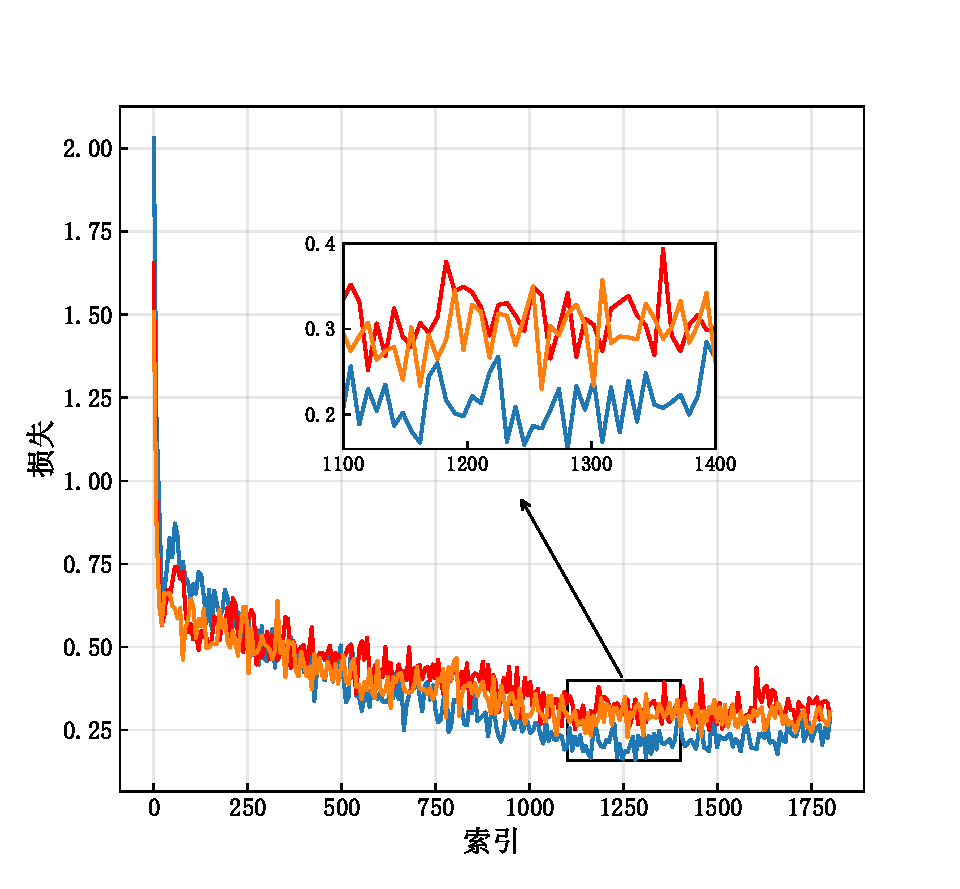
\includegraphics[width=3.2in] {fig9}
\caption{Convergence of MADQIN algorithm.}
\label{fig9}
\end{figure}

图 \ref{fig8} 和图 \ref{fig9} 分别给出了两种算法在迭代过程中的损失函数值。为使结果更具普适性，本文对三组损失结果进行了对比。可以看出，两种算法在迭代1200轮后均呈现出明显的收敛趋势，充分证明了两种算法均具备优异的性能稳定性。

\section{本章小结}
本文研究了存在非线性功率放大器（PA）与低分辨率模数转换器（ADC）场景下，CF‑mMIMO系统的上行数据传输问题，并推导出了可达用户速率的闭合表达式。研究结果表明，硬件性能会对系统性能产生显著影响。为补偿由非线性PA与低分辨率ADC造成的速率损失，本文提出一种基于深度强化学习的DMAGNN‑AC功率控制算法，以抑制来自其他用户的干扰。与全功率传输策略和DDPG算法相比，该算法可显著提升系统性能与最小用户速率下界。随后，本文利用MADQIN算法对ADC分辨率进行合理调整，使用户速率得到小幅提升。最后，通过深度强化学习算法验证了在CF‑mMIMO系统中使用低质量硬件的可行性。
